% The Slide Definitions
%document
\documentclass[10pt]{beamer}
%theme
\usetheme{metropolis}
% packages
\usepackage{color}
\usepackage{listings}
\usepackage[ngerman]{babel}
\usepackage[utf8]{inputenc}
\usepackage{multicol}


% color definitions
\definecolor{mygreen}{rgb}{0,0.6,0}
\definecolor{mygray}{rgb}{0.5,0.5,0.5}
\definecolor{mymauve}{rgb}{0.58,0,0.82}

\lstset{
    backgroundcolor=\color{white},
    % choose the background color;
    % you must add \usepackage{color} or \usepackage{xcolor}
    basicstyle=\footnotesize\ttfamily,
    % the size of the fonts that are used for the code
    breakatwhitespace=false,
    % sets if automatic breaks should only happen at whitespace
    breaklines=true,                 % sets automatic line breaking
    captionpos=b,                    % sets the caption-position to bottom
    commentstyle=\color{mygreen},    % comment style
    % deletekeywords={...},
    % if you want to delete keywords from the given language
    extendedchars=true,
    % lets you use non-ASCII characters;
    % for 8-bits encodings only, does not work with UTF-8
    literate={ä}{{\"a}}1 {ü}{{\"u}}1 {ö}{{\"o}}1 {Ä}{{\"A}}1 {Ü}{{\"U}}1 {Ö}{{\"O}}1 {ß}{{\ss{}}}1,
    % escapes umlauts
    frame=single,                    % adds a frame around the code
    keepspaces=true,
    % keeps spaces in text,
    % useful for keeping indentation of code
    % (possibly needs columns=flexible)
    keywordstyle=\color{blue},       % keyword style
    % morekeywords={*,...},
    % if you want to add more keywords to the set
    numbers=left,
    % where to put the line-numbers; possible values are (none, left, right)
    numbersep=5pt,
    % how far the line-numbers are from the code
    numberstyle=\tiny\color{mygray},
    % the style that is used for the line-numbers
    rulecolor=\color{black},
    % if not set, the frame-color may be changed on line-breaks
    % within not-black text (e.g. comments (green here))
    stepnumber=1,
    % the step between two line-numbers.
    % If it's 1, each line will be numbered
    stringstyle=\color{mymauve},     % string literal style
    tabsize=4,                       % sets default tabsize to 4 spaces
    % show the filename of files included with \lstinputlisting;
    % also try caption instead of title
    language = Python,
	showspaces = false,
	showtabs = false,
	showstringspaces = false,
	escapechar = ,
}

\def\ContinueLineNumber{\lstset{firstnumber=last}}
\def\StartLineAt#1{\lstset{firstnumber=#1}}
\let\numberLineAt\StartLineAt



\newcommand{\codeline}[1]{
	\alert{\texttt{#1}}
}


% Author and Course information
% This Document contains the information about this course.

% Authors of the slides
\author{Richard Müller, Tom Felber}

% Name of the Course
\institute{Python-Kurs}

% Fancy Logo 
\titlegraphic{\hfill\includegraphics[height=1.25cm]{../templates/fsr_logo_cropped}}



% Custom Bindings
% \newcommand{\codeline}[1]{
%	\alert{\texttt{#1}}
%}


% Presentation title
\title{Zahlen, Listen und Schleifen}
\date{28. Oktober 2021}

\usepackage{graphicx}

\begin{document}
	
\maketitle

\begin{frame}{Gliederung}
	\setbeamertemplate{section in toc}[sections numbered]
	\tableofcontents
\end{frame}


\section{Wiederholung}
\begin{frame}{Wiederholung}
	\textbf{Beim letzten Mal}:
	\begin{itemize}
		
		
		\item
		der Python Interpreter
		\item
		"Hallo Welt" mit der \alert{\texttt{print()}} Funktion 
		\item Interaktion mit dem Terminal mit \alert{\texttt{input()}}
		\item
		string Formatierung mit f-Strings
		\lstinputlisting[firstline=22,lastline=22]{resources/01_getting_started/string_format.py}
		\item \alert{\texttt{if / else / elif}} statements
		\item string methoden z.B. \alert{\texttt{isnumeric(), isupper()}}
		
		
	\end{itemize}
\end{frame}
% Problemfolie
\begin{frame}{Wiederholung}
	\begin{itemize}
		\item navigation mir dem Terminal in das richtige directory
		\begin{figure}
			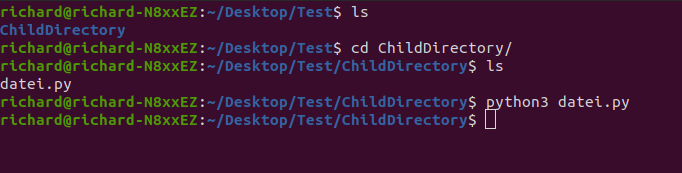
\includegraphics[width=\linewidth]{resources/02iteration/commandlinepython.png}
		\end{figure}
		
		\item
		starten eines python scripts
		\lstinputlisting[firstline=0,lastline=2]{resources/02iteration/python.txt}
		\item
		IndentationError: tritt z.B. auf, wenn Tabs und Leerzeichen nicht konsistent benutzt werden, oder bei flaschen Einrückungen
		\lstinputlisting[lastline=4]{resources/02iteration/bad_indentation.py}
		
	\end{itemize}
\end{frame}

\section{Zahlen}
\begin{frame}{Zahlen}
	\textbf{Die zwei Typen}
	\linebreak
	
	Python kennt zwei verschiedene Zahlentypen: 
	\begin{itemize}
		\item \alert{\texttt{int}} (Integer/Ganzzahl)
		\lstinputlisting[firstline=0,lastline=2]{resources/02iteration/numbers.py}
		\item \alert{\texttt{float}} (floating point number/Gleitkommazahl)
		\lstinputlisting[firstline=4,lastline=5]{resources/02iteration/numbers.py}
	\end{itemize}		
\end{frame}

\begin{frame}{Zahlen}
	\textbf{Mathematische Operationen}
	\linebreak

	Auf allen Zahlen sind verschiedene mathematische Operationen möglich:
	\lstinputlisting[firstline=7,lastline=12]{resources/02iteration/numbers.py}
	\begin{description}
		\item[\textbf{Achtung:}] Das Ergebnis wird bei der Division automatisch zu einem \alert{\texttt{float}} konvertiert, selbst dann, wenn es keinen Rest gibt.
	\end{description}
\end{frame}

\begin{frame}{Zahlen}
	Man kann auch bestehende Variablen einfach mit einem Ergebnis überschreiben, ohne eine neue Variable anlegen zu müssen:
	\lstinputlisting[firstline=14,lastline=16]{resources/02iteration/numbers.py}
	Dafür bietet Python eine Abkürzung:
	\lstinputlisting[firstline=18,lastline=21]{resources/02iteration/numbers.py}
\end{frame}

\begin{frame}{Zahlen}
	\textbf{Vergleichsoperationen}
	\linebreak
	
	Es sind mehrere Vergleichsoperationen möglich. Jede dieser Operationen resultiert in einem \alert{\texttt{bool}}:		
	\lstinputlisting[firstline=23,lastline=28]{resources/02iteration/numbers.py}
	Alle Ausdrücke in diesem Beispiel nehmen den Wert \alert{\texttt{True}} an.
\end{frame}

\section{Listen}
\begin{frame}{Listen - Initialisierung}
	Listen sind eine Datenstruktur vom Typ \alert{\texttt{list}}, eine geordnete Sammlung von Elementen.
	\lstinputlisting[firstline=0,lastline=6]{resources/02iteration/list.py}
	Indexierung startet in Python mit 0.
	\lstinputlisting[firstline=8,lastline=13]{resources/02iteration/list.py}
\end{frame}
\begin{frame}{Listen - append/remove}
	Listen bieten Funktionen zur einfachen Veränderung
	\lstinputlisting[firstline=2,lastline=2]{resources/02iteration/list.py}
	\lstinputlisting[firstline=15,lastline=18]{resources/02iteration/list.py}
	\lstinputlisting[firstline=19,lastline=21]{resources/02iteration/list.py}
	\lstinputlisting[firstline=23,lastline=26]{resources/02iteration/list.py}
\end{frame}

\section{for in Schleife}
\begin{frame}{for in Schleife}
	die Zahlen von 0 bis 999 durchgehen:
	\lstinputlisting[firstline=0,lastline=3]{resources/02iteration/for_loop.py}
	Objekte, die 'iterable' sind, elementweise durchgehen:
	\lstinputlisting[firstline=5,lastline=8]{resources/02iteration/for_loop.py}
	\lstinputlisting[firstline=10,lastline=13]{resources/02iteration/for_loop.py}
\end{frame}

\section{while Schleife}
	\begin{frame}{while Schleife}
		Die \alert{\texttt{while}}-Schleife prüft vor jeder Iteration, ob eine gegebene Bedingung den Wert \alert{\texttt{True}} besitzt:
		\lstinputlisting[firstline=0,lastline=2]{resources/02iteration/while_loop.py}
		Die Schleife bricht erst ab, wenn die Bedingung den Wert \alert{\texttt{False}} annimmt:
		\lstinputlisting[firstline=4,lastline=9]{resources/02iteration/while_loop.py}
	\end{frame}
	
	\begin{frame}{while Schleife}
	Die Bedingung muss während der Schleifenausführung verändert werden, sonst ist die Schleife endlos:
	\lstinputlisting[firstline=11,lastline=13]{resources/02iteration/while_loop.py}
	Wie bei der \alert{\texttt{for}}-Schleife gibt es auch hier das \alert{\texttt{break}}-Statement, womit man die Schleife auch unabhängig der Bedingung unterbrechen kann:
	\lstinputlisting[firstline=14,lastline=18]{resources/02iteration/while_loop.py}
	\end{frame}
\end{document}
